%\nonstopmode

\documentclass[11pt]{article}

\usepackage{mathenv}
\usepackage{cancel}
\usepackage{fullpage}
\usepackage{amsmath}
\usepackage{amsfonts}
\usepackage{ulem}
\usepackage{graphicx}
\usepackage{verbatim}
\usepackage{apalike}
\usepackage[usenames, dvipsnames]{color}
\usepackage[colorlinks=true, linkcolor=OliveGreen, citecolor=Purple]{hyperref}

\newcommand{\paperlink}[1]{\href{Documents/papers/#1.pdf}{\cite{#1}}}
\newcommand{\booklink}[2]{\href{Documents/books/#2.pdf}{\cite{#1}}}
\newcommand{\doh}{\partial}
\newcommand{\constant}{\text{ const. }}
\newcommand{\mc}{\mathcal}
\newcommand{\mb}{\mathbb}
\newcommand{\ds}{\displaystyle}
\newcommand{\ts}{\textstyle}

\allowdisplaybreaks

\begin{document}

\title{Inference on von Mises orientation maps}
\author{Carl Smith}
\date{May 10, 2012 - May 11, 2012}
\maketitle
%\tableofcontents

\section{Introduction}

So called low rank models, described in \paperlink{Smith_2012}, are continuous joint distributions $p(X)$ whose pairwise marginals $p(x_t,x_{t+1})$ and conditionals $p(x_{t+1}|x_t)$ can be expressed in terms of discrete random variables $Z$ coupling the adjacent components; e.g. $z_t$ couples $x_t$ and $x_{t+1}$, in a way that I'll explain in Section \ref{sec:low_rank_models}. Sampling, computation of moments, and smoothing of observations in these models are as efficient as in discrete Markov chains, provided that certain intermediate integrals can be computed.

One class of such models exploits the self-conjugacy of the von Mises distribution on the circle, which I'll describe in \ref{sec:von_mises_distribution}, to efficiently treat angular variables and data. For example, \paperlink{Smith_2012} use this kind of smoother to estimate joint angle movement from motion capture data. Other examples are imaginable, even in higher dimensions with a generalized form of the von Mises. In this note, in Section \ref{sec:loopy_orientation_map_model}, I'm describing a loopy low rank von Mises model to sample and estimate orientation maps like those found in primary visual cortex. For another approach to modeling orientation maps using Gaussian processes, see \paperlink{Macke_2009}.

Because this orientation map model is loopy we can't do exact inference by the forward backward algorithm. However, we can do block-wise Gibbs sampling to speed up mixing compared to simple point-wise sampling of each variable. In principle both have the same scaling of processing time with the rank of the model, which will be defined in Section \ref{sec:low_rank_models}. In Section \ref{sec:samples_and_reconstructions}, I'll show some output from the model: samples from the prior and reconstructions from the posterior given artificially corrupted samples.


\section{Low rank models}
\label{sec:low_rank_models}

Low rank models are joint distributions whose structure allows for fast exact inference in settings where standard models such as hidden Markov models and linear Gaussian models are not applicable. We can perform fast inference on any low rank model with a tree structure, i.e. without loops, and beyond that low rank inference may be used in the context of block-wise sampling of loopy distributions. 

\begin{figure}[h]
\centering
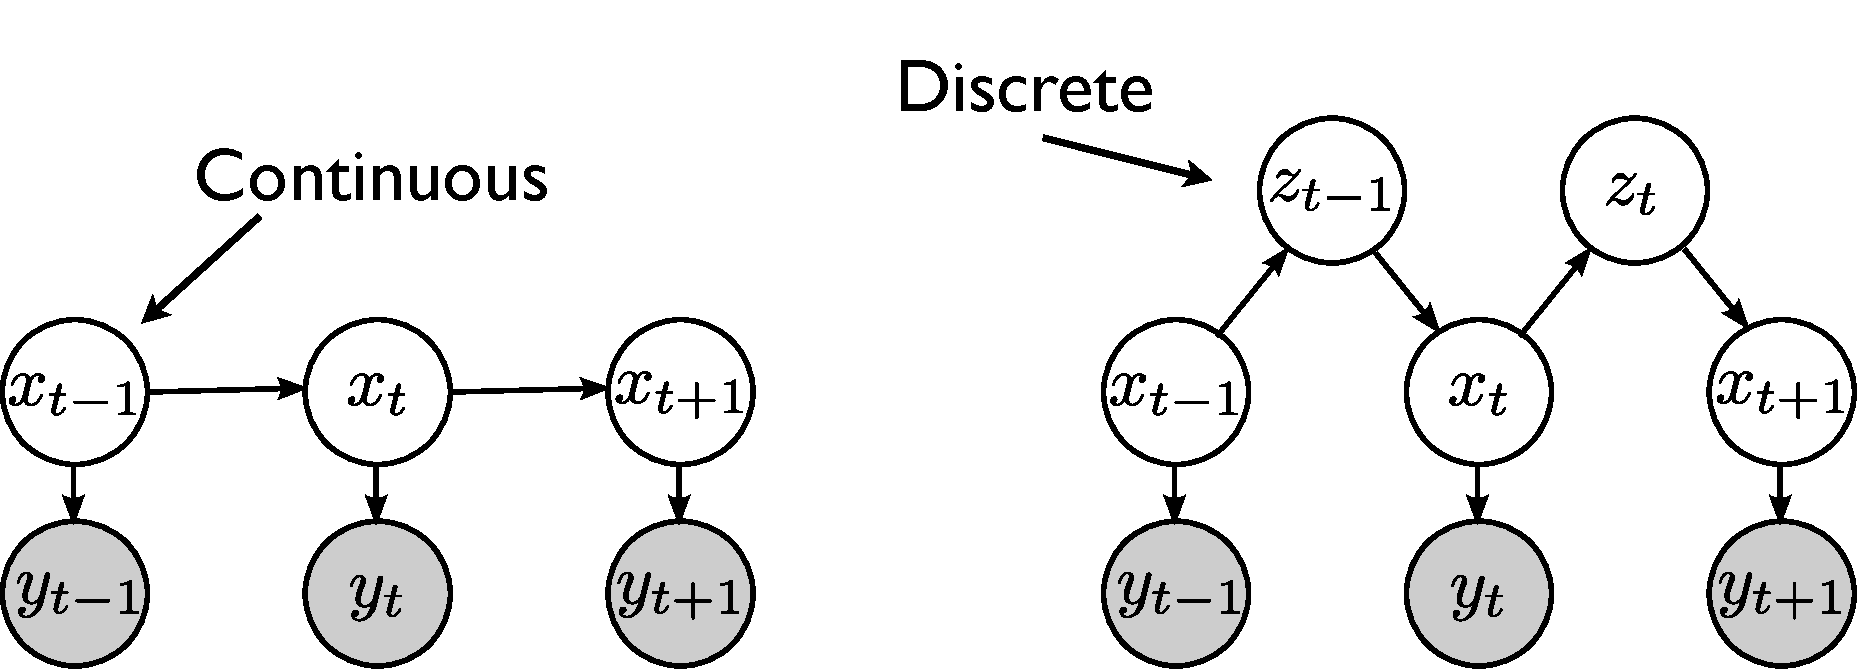
\includegraphics[scale=0.35]{../fig/aux_vars}
\caption{On the left, a general chain structured distribution of latent variables $X$ and observations $Y$. On the right, such a model expressed in terms of discrete auxiliary variables $Z$.}
\label{fig:aux_vars}
\end{figure}

Suppose, for simplicity, that we are interested in a distribution $p(X)$ over some latent variables $X$, whose dependence structure forms a chain. (More generally, consider the posterior of $X$ given some observations $Y$.) Suppose that $X$ is continuous but with non-Gaussian marginals, so that neither HMMs nor linear Gaussian models are appropriate. But suppose that the dependence structure of $X$ can be expressed in terms of latent variables $Z$ with some small discrete state space, where each neighboring pair of continuous $x$'s is coupled through some discrete variable $z$, as shown in Figure \ref{fig:aux_vars}. The graph on the left has the form

\begin{align*}
p(X|Y)=p(x_1)\prod_{t=1}^{T-1}\left[\vphantom{\sum_{i}^{J}}p(x_{t+1}|x_t)\right]p(y_t|x_t).
\end{align*}

\noindent The graph on the right, as the distribution $p(X|Y)$, has the same form, but it can also be expressed as

\begin{align*}
p(X|Y)=p(x_1)\prod_{t=1}^{T-1}\left[\sum_{z_t}^{R_t}p(z_t|x_t)p(x_{t+1}|z_t)\right]p(y_t|x_t)
\end{align*}

\noindent where we have replaced the transition kernel between $x_t$ and $x_{t+1}$ with a sum over $z_t$, which is a discrete variable with few states. This looks like the decomposition of a matrix into rank-one matrices, by singular value decomposition, for example, except that $p(z_t | x_t)$ and $p(x_{t+1} | z_t)$ are continuous functions, not vectors. Nonetheless, we can consider such a potential function to be in some sense a truncated approximation to some more complicated or ``high rank" function, where $R_t$ here is the rank of the truncated function, which is just the size of the state space of $z_t$. If the $x$'s were discrete random variables, then this equation would represent a discrete Markov chain in which the transition densities are of rank $R_t$, and inference in this kind of Markov chain is relatively easy, since multiplication by low-rank matrices is relatively cheap.

The key idea here is that exact inference of the Markov chain $X$ is tractable even in the general, non-discrete case. In these distributions, $X$ can be marginalized out, leaving a Markov chain in $Z$ only, where exact inference is tractable by the forward backward algorithm.

\begin{align*}
p(Z) &\propto \int dx_1 p(z_1|x_1) \int dx_2 p(x_2|z_1) p(z_2|x_2) \int dx_3 p(x_3|z_2) p(z_3|x_3) \cdots \int dx_T p(x_T|z_{T-1})
\end{align*}

\noindent (I've omitted the factors $p(y_t|x_t)$ here, for brevity. They may be considered absorbed into the respective factors $p(z_t|x_t)$.) The corresponding forward variables are shown here. These expressions, and similar ones for the backward variables, can be derived by induction on t.

\begin{align*}
A_1^{(z_1)} &= \int dx_1 p(x_1) p(z_1|x_1) p(y_1|x_1)\\
A_t^{(z_t)} &= \sum_{z_{t-1}}^{R_{t-1}} A_{t-1}^{(z_{t-1})} \int dx_t p(x_t|z_{t-1}) p(z_t|x_t) p(y_t|x_t)
\end{align*}

\noindent But given $Z$, the $x$'s are independent, so we can easily compute exact marginals or samples from $p(X)$ as well.

\begin{align*}
p(x_t|Y) \propto \sum_{z_{t-1}}^{R_{t-1}} A_{t-1}^{(z_{t-1})} \sum_{z_t}^{R_t} B_{t+1}^{(z_t)} p(x_t|z_{t-1}) p(z_t|x_t) p(y_t|x_t)
\end{align*}

\noindent The marginal distribution of $x_t$ can be exactly expressed in terms of the neighboring forward backward variables of $Z$. So we’re doing discrete forward backward to perform inference on continuous variables.

An important thing to note is that we can compute these exactly so long as the inner products here are evaluable:

\begin{align*}
\int dx_t p(x_t|z_{t-1}) p(z_t|x_t) p(y_t|x_t)
\end{align*}

\noindent These integrals correspond to the inner products of left and right singular vectors in the discrete Markov chain analogy, of which there are few kept from the ``full rank" density. Also, note that we need only compute these inner product integrals once. They can be tabulated before inference begins.

If we can compute the inner product integrals, analytically or numerically, then inference takes $O(R^2 T)$ time and $O(RT)$ storage (assuming a fixed $R_t=R$). If the potential function basis functions $p(z_t | x_t)$ and $p(x_{t+1} | z_t)$ are such that $p(x_{t+1}|x_t)$ is effectively banded, as would often be the case in smoothing applications, then the speed would scale linearly with the rank of the potentials as opposed to quadratically, further speeding up inference.

\section{The von Mises distribution and smoothing potential}
\label{sec:von_mises_distribution}

\subsection{The von Mises distribution}

The von Mises distribution is popular for modeling one-dimensional angular data, largely because the necessary normalization factors can be computed easily, and furthermore it is conjugate to itself, like the Gaussian. On the unit circle, the von Mises distribution can be parametrized by the ``mean" angle $\phi$ where the mode of the density resides:
%
\begin{align*}
f(x|\phi,\kappa) &= \frac{e^{\kappa\cos(x-\phi)}}{2\pi I_0(\kappa)}
\end{align*}

\noindent where $I_0(x)$ is the order 0 modified Bessel function. (Assume throughout that $\kappa$ is fixed.) Instead, however, consider the unit vector $\mathbf{x}$ from the circle's center to the point on the perimeter an angle $x$ away from the $x$-axis. Similarly define $\mathbf{\mu}$ to be the vector with tail at the circle's center and point on the perimeter making the angle $\phi$ with the $x$-axis. This we may write
%
\begin{align*}
f(\mathbf{x}|\mathbf{\mu},\kappa) = \frac{e^{\kappa \mathbf{\mu}^T \mathbf{x}}}{2\pi I_0(\kappa)}.
\end{align*}

\noindent This is more generally an expression for the $p$-dimensional von Mises-Fisher distribution on the surface of the $p$-sphere, where $\mathbf{x}$ and $\mu$ are $p$-vectors and where $(2\pi I_0(\kappa))^{-1}$ is replaced by the more general normalization constant 
%
\begin{align*}
C_p(\kappa)=\frac{\kappa^{p/2-1}}{(2\pi)^{p/2} I_{p/2-1}(\kappa)}.
\end{align*}

\noindent In particular,
%
\begin{align*}
C_3(\kappa)=\frac{\kappa}{4\pi\sinh\kappa}
\end{align*}

A fairly simple algorithm for sampling from the von Mises distribution is described in \paperlink{Best_1979} and implemented in the Circular Statistics Toolbox written for MATLAB by Peter Berens and described in \paperlink{Berens_2009}. Said toolbox also includes useful functions such as evaluation of the von Mises pdf.

\subsection{The von Mises smoothing prior}

Suppose we have a time series of angular variables $X$ that we know to vary gradually. Then we may want to model $X$ with a low rank chain distribution that couples neighboring $x$'s in such a way both that smoothness is imposed on $X$ and that the necessary inner products are very easy to compute. On such model is
%
\begin{align*}
p(X)\propto\prod_t\sum_{i=0}^Re^{\kappa_t\cos\left(x_t-\frac{2\pi i}{R+1}\right)}e^{\kappa_t\cos\left(x_{t+1}-\frac{2\pi i}{R+1}\right)}
\end{align*}

\noindent For each time step $t$, this can be viewed as, and is, a superposition of unimodal functions of $x_t$ and $x_{t+1}$, each peaked at $x_t=x_{t+1}=\frac{2\pi i}{R+1}$ for $i=1,\cdots,R$, as illustrated in Figure \ref{fig:vm_bumps}.

\begin{figure}[h]
\centering
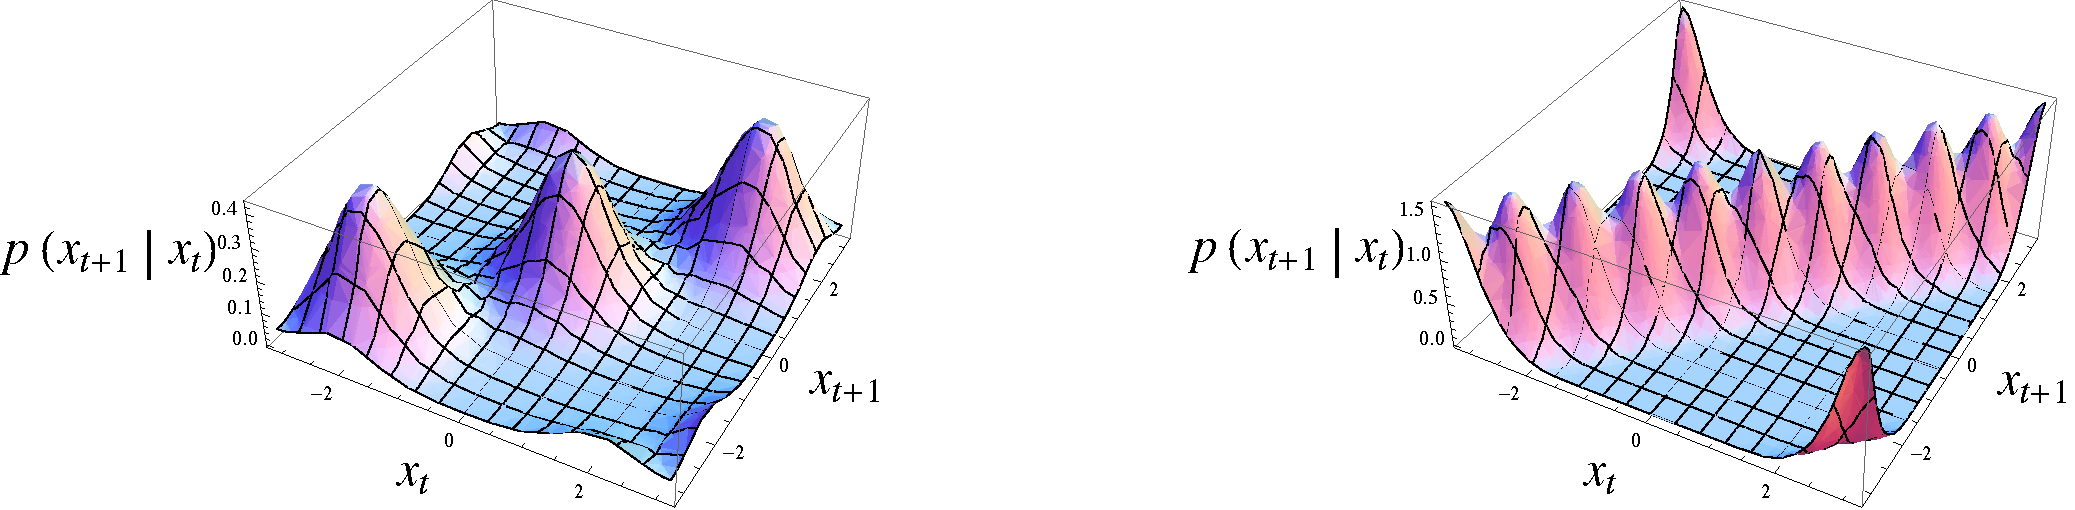
\includegraphics[scale=0.40]{../fig/vm_bumps}
\caption{The von Mises smoother transition kernel, shown for rank $R=3$ (left) and $R=10$ (right), where $\kappa_t:=R$ in each case.}
\label{fig:vm_bumps}
\end{figure}

\section{Loopy orientation map model}
\label{sec:loopy_orientation_map_model}

On the cortical surface, we know that in many cases nearby columns of cells have similar tuning properties, so that if we want to estimate the tuning properties of some of these columns that we observe simultaneously then it makes sense to share information across neurons by smoothing.  In primary visual cortex, the preferred orientation is usually a smooth function of position. See \paperlink{Ohki_2006} for an example of analysis of orientation preference data. 

\subsection{Smooth prior and posterior distributions of an orientation map}

(Notation change: $Z$ is now observations, not auxiliary variables, which will go by $k$, $l$, and $m$.) Figure \ref{fig:som_gm0} is a graphical model of the orientation preferences of an array of cortical columns.  (The graphical model has rows and columns, and the nodes represent columns of cells. I hope it's clear which kind of column I'm referring to in a given context. I'll try to stick to calling the columns of cells {\it nodes}). Let $o_{i,j}$ denote the preferred orientation of the node at position $(i,j)$.  We make a noisy observation $z_{i,j}$ of each node's orientation preference. Then we have that
%
\begin{align}
p(O,Z) &= p(O) p(Z|O) \notag \\
p(Z|O) &= \prod_{i,j} p( z_{i,j} | o_{i,j} ).
\end{align}

We need a smoothing prior $p(O)$. One convenient choice is to use a low rank spatial prior.
%
\begin{align}
p(O) &= \prod_{i,j} p(o_{i,j+1}|o_{i,j}) p(o_{i+1,j}|o_{i,j})
\end{align}

\noindent Here the term $p(o_{i,j+1}|o_{i,j})$ penalizes roughness in the horizontal direction, and $p(o_{i+1,j}|o_{i,j})$ penalizes the vertical direction. The following edge potentials serve to smooth orientation maps, coupling adjacent nodes to keep their values similar:
%
\begin{align}
p(o_{i,j}|o_{i-1,j}) &\propto \sum_{k=0}^R e^{\kappa \cos\left(o_{i-1,j}-\frac{2\pi k}{R+1}\right)} e^{\kappa \cos\left(o_{i,j}-\frac{2\pi k}{R+1}\right)} \\
p(o_{i,j}|o_{i,j-1}) &\propto \sum_{k=0}^R e^{\kappa \cos\left(o_{i,j-1}-\frac{2\pi k}{R+1}\right)} e^{\kappa \cos\left(o_{i,j}-\frac{2\pi k}{R+1}\right)} \notag
\end{align}
%
\begin{figure}[h]
\centering
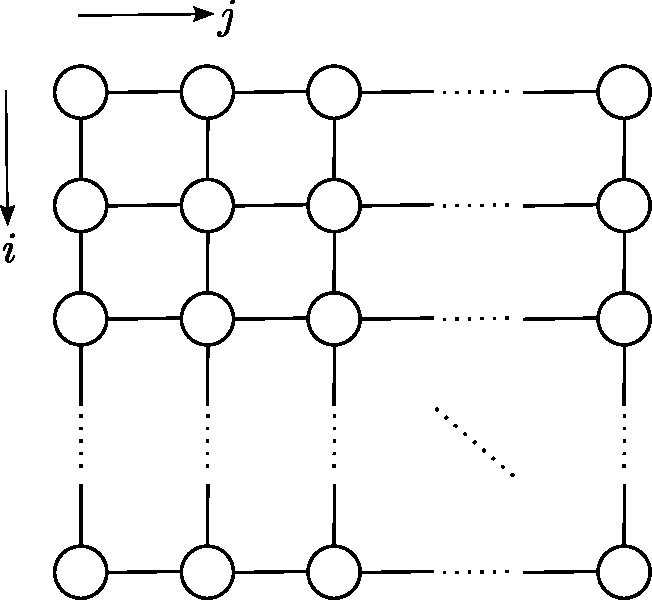
\includegraphics[scale=0.50]{../fig/col_grid_gm}
\caption{A graphical model of orientation selectivity, omitting observed nodes and their dependencies.}
\label{fig:som_gm0}
\end{figure}

\noindent We can suppose that each node has a flat prior $p(o_{i,j})$, as we do here for simplicity, or we can suppose von Mises priors about set modes. (I'm being a bit fast and loose about whether this is a Markov random field or a Bayesian net, dealing with edge potentials as if they were transition probabilities. Hopefully the meaning is clear and I don't think there's anything illogical.) Throughout, the concentration parameter $\kappa$ is assumed to be fixed, though this assumption can be relaxed. With the observations included the graphical model may be depicted as in Figure \ref{fig:som_gm2}, where the small black circles denote the observations which have probability
%
\begin{align}
p(z_{i,j}|o_{i,j}) &\propto e^{\kappa \cos(z_{i,j}-o_{i,j})}.
\end{align}

\begin{figure}[h]
\centering
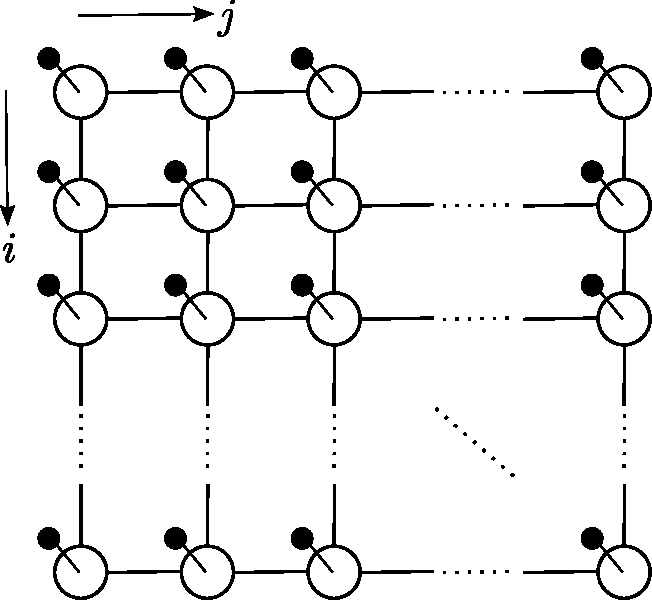
\includegraphics[scale=0.50]{../fig/col_grid_gm_obs}
\caption{A graphical model of orientation selectivity, including observed nodes and their dependencies.}
\label{fig:som_gm2}
\end{figure}

\subsection{The conditional distribution of a column}

Define $\mathbf{r}_k$ to be the unit vector that makes an angle of $\frac{2\pi k}{R+1}$ with the $x$-axis. Define $\mathbf{o}_{i,j}$ to be the vector that makes an angle of $o_{i,j}$ with the $x$-axis. Define $\mathbf{z}_{i,j}$ to be the unit vector that makes an angle of $z_{i,j}$ with the $x$-axis. Suppose that was have marginal estimates for every node and that we wish to block-wise draw a sample from the $j^{th}$ column. Without loss of generality, assume $1<j<N$ where $N$ is the number of columns and $M$ the number of rows. The conditional distribution of the $j^{th}$ column given the rest of the nodes and given the observations is

\begin{align}
P_j &\equiv p(O_{1:M,j}|O\backslash O_{1:M,j},Z) \\
&= p(O_{1:M,j}|O_{1:M,j-1},O_{1:M,j+1},Z_{1:M,j}) \notag \\
&= p(o_{1,j}|o_{1,j-1},o_{1,j+1},z_{1,j}) \prod_{i=2}^M p(o_{i,j}|o_{i-1,j},o_{i,j-1},o_{i,j+1},z_{i,j}). \notag
\end{align}

\noindent This first factor is
%
\begin{align}
\label{eq:first_factor}
p(o_{1,j}|o_{1,j-1},o_{1,j+1},z_{1,j}) &\propto p(o_{1,j-1}) p(o_{1,j}|o_{1,j-1})p(o_{1,j+1}|o_{1,j})p(z_{1,j}|o_{1,j}) \\
&\propto p(o_{1,j}|o_{1,j-1})p(o_{1,j+1}|o_{1,j})p(z_{1,j}|o_{1,j}) \notag \\
&\propto \sum_{k=0}^R e^{\kappa \mathbf{r}_k^T \mathbf{o}_{1,j-1}} e^{\kappa \mathbf{r}_k^T \mathbf{o}_{1,j}}
\sum_{k'=0}^R e^{\kappa \mathbf{r}_{k'}^T \mathbf{o}_{1,j}} e^{\kappa \mathbf{r}_{k'}^T \mathbf{o}_{1,j+1}}
\cdot e^{\kappa \mathbf{z}_{1,j}^T\mathbf{o}_{1,j} }. \notag
\end{align}

\noindent The second factor is
%
\begin{align*}
p(o_{i,j}|o_{i-1,j},o_{i,j-1},o_{i,j+1},z_{i,j}) &\propto p(o_{i,j-1}) p(o_{i-1,j}) p(o_{i,j}|o_{i,j-1})p(o_{i,j+1}|o_{i,j})p(z_{i,j}|o_{i,j}) \\
&\propto p(o_{i,j}|o_{i,j-1})p(o_{i,j+1}|o_{i,j})p(z_{i,j}|o_{i,j}) \\
&\propto \sum_{k=0}^R e^{\kappa \mathbf{r}_k^T \mathbf{o}_{i,j-1}} e^{\kappa \mathbf{r}_k^T \mathbf{o}_{i,j}}
\sum_{k'=0}^R e^{\kappa \mathbf{r}_{k'}^T \mathbf{o}_{i,j}} e^{\kappa \mathbf{r}_{k'}^T \mathbf{o}_{i,j+1}}
\cdot e^{\kappa \mathbf{z}_{i,j}^T\mathbf{o}_{i,j} }.
\end{align*}

\noindent Putting these together, the conditional distribution is

\begin{align}
P_j \propto \sum_{k=0}^R &e^{\kappa \mathbf{r}_k^T \mathbf{o}_{1,j-1}} e^{\kappa \mathbf{r}_k^T \mathbf{o}_{1,j}}
\sum_{k'=0}^R e^{\kappa \mathbf{r}_{k'}^T \mathbf{o}_{1,j}} e^{\kappa \mathbf{r}_{k'}^T \mathbf{o}_{1,j+1}}
\cdot e^{\kappa \mathbf{z}_{1,j}^T\mathbf{o}_{1,j} } \times \\
&\prod_{i=2}^T \sum_{k''=0}^R e^{\kappa \mathbf{r}_{k''}^T\mathbf{o}_{i,j-1}} e^{\kappa \mathbf{r}_{k''}^T\mathbf{o}_{i,j}}
\sum_{k'''=0}^R e^{\kappa \mathbf{r}_{k'''}^T\mathbf{o}_{i,j}} e^{\kappa \mathbf{r}_{k'''}^T\mathbf{o}_{i,j+1}}. \notag
\end{align}

\subsection{Sampling a column block-wise by the filter forward sample backward algorithm}

Along column $j$, starting from the top ($i=1$), we compute forward variables each corresponding to a particular value of the auxiliary value $k_i$ that connects $o_{i,j}$ to $o_{i+1,j}$. It is helpful to have the joint factor graph representation in Figure \ref{fig:som_gm3} in mind. In this figure, the index of summation over an auxiliary variable labels the factor corresponding to that auxiliary variable.

\begin{align}
A_1^{(k_1)} &= \int do_{1j} p(o_{1j}) p(k_1|o_{1j}) p(z_{1j}|o_{1j}) \notag \\
&= \frac{1}{\mc{Z}_{A,1}} \int do_{1j} \left( \sum_{l_1=0}^R e^{\kappa \mathbf{r}_{l_1}^T \mathbf{o}_{1,j-1}}e^{\kappa \mathbf{r}_{l_1}^T \mathbf{o}_{1j}} \sum_{m_1=0}^R e^{\kappa \mathbf{r}_{m_1}^T \mathbf{o}_{1j}} e^{\kappa \mathbf{r}_{m_1}^T \mathbf{o}_{1,j+1}} \right) e^{\kappa \mathbf{r}_{k_1}^T \mathbf{o}_{1j}} e^{\kappa \mathbf{z}_{1j}^T\mathbf{o}_{1j}} \notag \\
&= \frac{1}{\mc{Z}_{A,1}}  \sum_{l_1=0}^R \sum_{m_1=0}^R e^{\kappa (\mathbf{r}_{l_1}^T\mathbf{o}_{1,j-1}+\mathbf{r}_{m_1}^T\mathbf{o}_{1,j+1})} \int do_{1j} e^{\kappa(\mathbf{r}_{l_1}+\mathbf{r}_{m_1}+\mathbf{r}_{k_1}+\mathbf{z}_{1j})^T\mathbf{o}_{1j}} \notag \\
&= \frac{1}{\mc{Z}_{A,1}}  \sum_{l_1=0}^R \sum_{m_1=0}^R e^{\kappa (\mathbf{r}_{l_1}^T\mathbf{o}_{1,j-1}+\mathbf{r}_{m_1}^T\mathbf{o}_{1,j+1})} \frac{1}{C_3(\kappa\cdot ||\mathbf{r}_{l_1}+\mathbf{r}_{m_1}+\mathbf{r}_{k_1}+\mathbf{z}_{1j}||)} \\[5mm]
A_i^{(k_i)} &= \sum_{k_{i-1}=0}^R A_{i-1}^{(k_{i-1})} \int do_{i,j} p(o_{i,j}|k_{i-1})p(k_i|o_{i,j})p(z_{i,j}|o_{i,j}) \notag \\
&= \frac{1}{\mc{Z}_{A,i}}  \sum_{k_{i-1}=0}^R A_{i-1}^{(k_{i-1})} \int do_{i,j} \left( \sum_{l_i=0}^R e^{\kappa\mathbf{r}_{l_i}^T\mathbf{o}_{i,j-1}} e^{\kappa\mathbf{r}_{l_i}^T\mathbf{o}_{i,j}} \sum_{m_i=0}^R e^{\kappa\mathbf{r}_{m_i}^T\mathbf{o}_{i,j}} e^{\kappa\mathbf{r}_{m_i}^T\mathbf{o}_{i,j+1}}\right) e^{\kappa \mathbf{r}_{k_{i-1}}^T \mathbf{o}_{i,j}} e^{\kappa \mathbf{r}_{k_i}^T \mathbf{o}_{i,j}} \notag \\
&= \frac{1}{\mc{Z}_{A,i}}  \sum_{k_{i-1}=0}^R A_{i-1}^{(k_{i-1})} \sum_{l_i=0}^R \sum_{m_i=0}^R e^{\kappa\left(\mathbf{r}_{l_i}^T\mathbf{o}_{i,j-1}+\mathbf{r}_{m_i}^T\mathbf{o}_{i,j+1}\right)} \int do_{i,j} e^{\kappa(\mathbf{r}_{l_i}+\mathbf{r}_{m_i}+\mathbf{r}_{k_{i-1}}+\mathbf{r}_{k_i}+\mathbf{z}_{i,j})^T\mathbf{o}_{i,j}} \notag \\
&= \frac{1}{\mc{Z}_{A,i}}  \sum_{k_{i-1}=0}^R A_{i-1}^{(k_{i-1})} \sum_{l_i=0}^R \sum_{m_i=0}^R e^{\kappa\left(\mathbf{r}_{l_i}^T\mathbf{o}_{i,j-1}+\mathbf{r}_{m_i}^T\mathbf{o}_{i,j+1}\right)} \frac{1}{C_3(\kappa\cdot ||\mathbf{r}_{l_i}+\mathbf{r}_{m_i}+\mathbf{r}_{k_{i-1}}+\mathbf{r}_{k_i}+\mathbf{z}_{i,j}||)}
\end{align}

\begin{figure}[h]
\centering
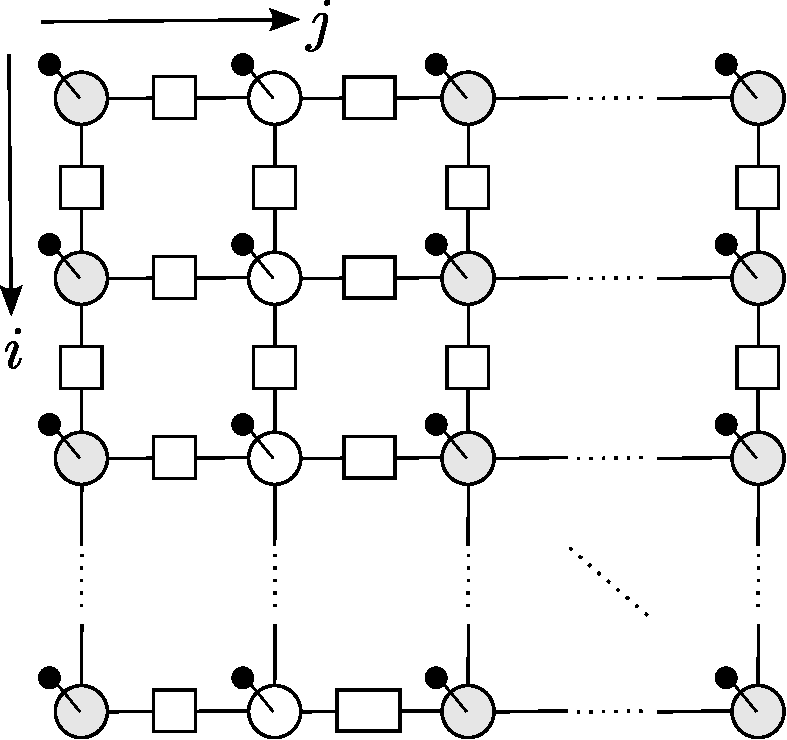
\includegraphics[scale=0.55]{../fig/col_grid_gm_factors}
\caption{A graphical model of orientation selectivity, including observed nodes and auxiliary variables and their dependencies, drawing attention to a forward backward run on the second column from the left. The shaded nodes' values are held as constants, as are the observations. At each step of the forward recursion, to each possible value of $k_i$ corresponds a forward variable $A_i^{(k_i)}$.}
\label{fig:som_gm3}
\end{figure}

\noindent where the normalization constant for each time step $t$ is computed by summing over the unnormalized variables $A_t^{(k_t)}$ with respect to $k_t$.  With these variables in hand we can use the standard filter forward sample backward algorithm of hidden Markov model theory to generate samples from the prior (with observations set to zero) or posterior. Here's how: first we want to sample $o_{j,M}$ given $o_{j-1,M}$, $o_{j+1,M}$, and $z_{j,M}$. That marginal distribution is 
%
\begin{align*}
	p(o_{M,j}&|o_{M,j-1},o_{M,j+1},z_{M,j}) \\
	&=\sum_k A_{M-1}^{(k)} e^{\kappa\mathbf{r}_k^T\mathbf{o}_{M,j}}\sum_{k'=0}^R e^{\kappa \mathbf{r}_{k'}^T \mathbf{o}_{M,j-1}} e^{\kappa \mathbf{r}_{k'}^T\mathbf{o}_{M,j}} \sum_{k''=0}^R e^{\kappa \mathbf{r}_{k''}^T \mathbf{o}_{M,j+1}} e^{\kappa \mathbf{r}_{k''}^T\mathbf{o}_{M,j}} \cdot e^{\kappa \mathbf{z}_{M,j}^T \mathbf{o}_{M,j}} \\
	&=\sum_k A_{M-1}^{(k)} \sum_{k'=0}^R e^{\kappa \mathbf{r}_{k'}^T \mathbf{o}_{M,j-1}} \sum_{k''=0}^R e^{\kappa \mathbf{r}_{k''}^T \mathbf{o}_{M,j+1}}\left( e^{\kappa\mathbf{r}_k^T\mathbf{o}_{M,j}} e^{\kappa \mathbf{r}_{k'}^T\mathbf{o}_{M,j}} e^{\kappa \mathbf{r}_{k''}^T\mathbf{o}_{M,j}} e^{\kappa \mathbf{z}_{M,j}^T \mathbf{o}_{M,j}}\right) 
\end{align*}

Next up is the conditional distribution used to sample the rest of the elements of the column:
%
\begin{align*}
	p(o_{m,j}&|o_{m+1,j},o_{m,j-1},o_{m,j+1},z_{m,j}) \\
	&=\sum_k A_{m-1}^{(k)} \sum_{k'=0}^R e^{\kappa \mathbf{r}_{k'}^T \mathbf{o}_{m,j-1}} \sum_{k''=0}^R e^{\kappa \mathbf{r}_{k''}^T \mathbf{o}_{m,j+1}}\left( e^{\kappa\mathbf{r}_k^T\mathbf{o}_{m,j}} e^{\kappa \mathbf{r}_{k'}^T\mathbf{o}_{m,j}} e^{\kappa \mathbf{r}_{k''}^T\mathbf{o}_{m,j}} e^{\kappa \mathbf{z}_{m,j}^T \mathbf{o}_{m,j}}\right) \times \\
	&\sum_{k'''=0}^{R} e^{\kappa \mathbf{r}_{k'''}^T \mathbf{o}_{m+1,j}} e^{\kappa \mathbf{r}_{k'''}^T \mathbf{o}_{m,j}} \\
	&=\sum_k A_{m-1}^{(k)} \sum_{k'=0}^R e^{\kappa \mathbf{r}_{k'}^T \mathbf{o}_{m,j-1}} \sum_{k''=0}^R e^{\kappa \mathbf{r}_{k''}^T \mathbf{o}_{m,j+1}} \sum_{k'''=0}^{R} e^{\kappa \mathbf{r}_{k'''}^T \mathbf{o}_{m+1,j}} \times \\
	&\left( e^{\kappa\mathbf{r}_k^T\mathbf{o}_{m,j}} e^{\kappa \mathbf{r}_{k'}^T\mathbf{o}_{m,j}} e^{\kappa \mathbf{r}_{k''}^T\mathbf{o}_{m,j}} e^{\kappa \mathbf{r}_{k'''}^T \mathbf{o}_{m,j}}e^{\kappa\mathbf{z}_{m,j}^T \mathbf{o}_{m,j}} \right) 
\end{align*}

\subsection{Computing marginal distributions by the forward backward algorithm}

As above with the forward variables we may derive backward variables:
%
\begin{align}
B_M^{(k_{M-1})} &= \int do_{M,j} p(o_{M,j}|k_{M-1,j}) p(z_{M,j}|o_{M,j}) \notag \\
&= \frac{1}{\mc{Z}_{B,M}} \sum_{l_{M}=0}^R \sum_{m_{M}=0}^R 
e^{\kappa\left( \mathbf{r}_{l_{M}}^T \mathbf{o}_{M,j-1}+
\mathbf{r}_{m_{M}}^T \mathbf{o}_{M,j+1}\right)}
\frac{1}{C_3(\kappa\cdot ||\mathbf{r}_{l_{M}}+\mathbf{r}_{m_{M}}+\mathbf{r}_{k_{M-1}}+\mathbf{z}_{M,j}||)} \\
B_i^{k_{i-1}} &= \sum_{k_i=0}^R B_{i+1}^{k_i} \int do_{i,j} p(o_{i,j}|k_{i-1}) p(k_i|o_{i,j}) p(z_{i,j}|o_{i,j}) \notag \\
&= \frac{1}{\mc{Z}_{B,i}}  \sum_{k_i=0}^R B_{i+1}^{k_i}
\sum_{l_{i}=0}^R \sum_{m_{i}=0}^R 
e^{\kappa\left( \mathbf{r}_{l_{i}}^T \mathbf{o}_{i,j-1}+
\mathbf{r}_{m_{i}}^T \mathbf{o}_{i,j+1}\right)}
\frac{1}{C_3(\kappa\cdot ||\mathbf{r}_{l_{i}}+\mathbf{r}_{m_{i}}+\mathbf{r}_{k_{i-1}}+\mathbf{r}_{k_{i}}+\mathbf{z}_{i,j}||)}
\end{align}

\noindent With these in hand we are equipped to write down the marginal distribution of any given node:

\begin{align}
p(o_{i,j}|Z) &\propto \sum_{k_{i-1}=0}^R A_{i-1}^{(k_{i-1})} \sum_{k_i=0}^R B_{i+1}^{(k_{i})} p(o_{i,j}|k_{i-1}) p(k_i|o_{i,j}) p(z_{i,j}|o_{i,j}) \notag \\
&= \sum_{k_{i-1}=0}^R A_{i-1}^{(k_{i-1})} \sum_{k_i=0}^R B_{i+1}^{(k_{i})} \left( \sum_{l_i=0}^R e^{\kappa\mathbf{r}_{l_i}^T\mathbf{o}_{i,j-1}} e^{\kappa\mathbf{r}_{l_i}^T\mathbf{o}_{i,j}} \sum_{m_i=0}^R e^{\kappa\mathbf{r}_{m_i}^T\mathbf{o}_{i,j}} e^{\kappa\mathbf{r}_{m_i}^T\mathbf{o}_{i,j+1}}\right) \times \\[2mm]
&\;\;\;\;\;\;\;e^{\kappa \mathbf{r}_{k_{i-1}}^T \mathbf{o}_{i,j}} e^{\kappa \mathbf{r}_{k_i}^T \mathbf{o}_{i,j}}. \notag
\end{align}

\noindent And here it becomes clear that while inference time scales quadratically with rank in a tree structured low rank model, here the scaling will be quartic, which obviously limits how high we can tune the rank, and therefore how uniform we can make the smoothing. As an example, simulations with rank 10 and $10^4$ nodes take several hours.

\section{Samples, reconstructions, and code}
\label{sec:samples_and_reconstructions}

Figure \ref{fig:sample_1} is a sample from the von Mises orientation preference model for rank $R=5$. More samples, along with reconstructions of maps from noisy data, can be found in the Git folder as movies. The Git folder also includes code for sampling from the prior and reconstructing maps from noisy observations. The code actually does not implement the block-wise approach but rather simply samples point-wise. My mistake. I might upload block-wise code soon.

\begin{figure}[h]
\centering
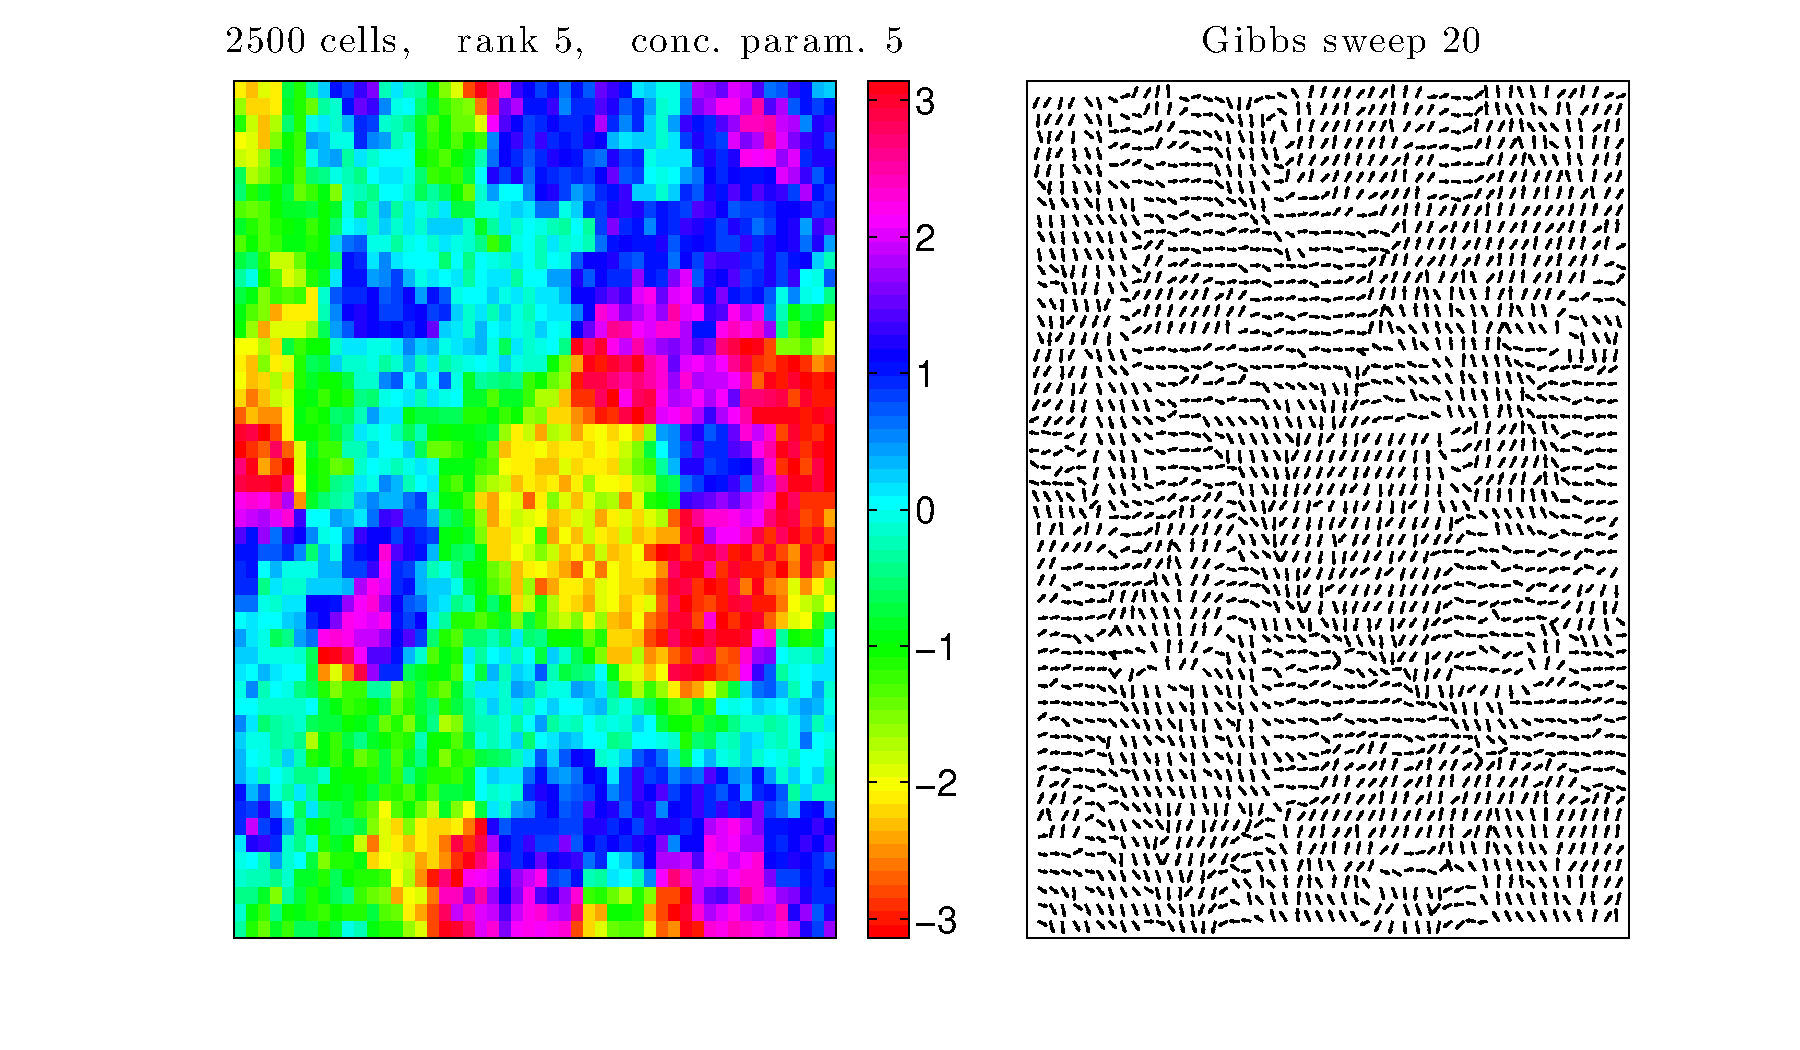
\includegraphics[scale=0.5]{../fig/sample__N_1024__R_5__kq_5__ky_5__nG_20}
\caption{A sample $50\times50$ grid of angles drawn from the von Mises orientation map prior with rank $R=5$ and $\kappa_t=5\;\;\forall t$. Twenty Gibbs sweeps were made.}
\label{fig:sample_1}
\end{figure}

\bibliographystyle{apalike}
\bibliography{refs}
\end{document}
